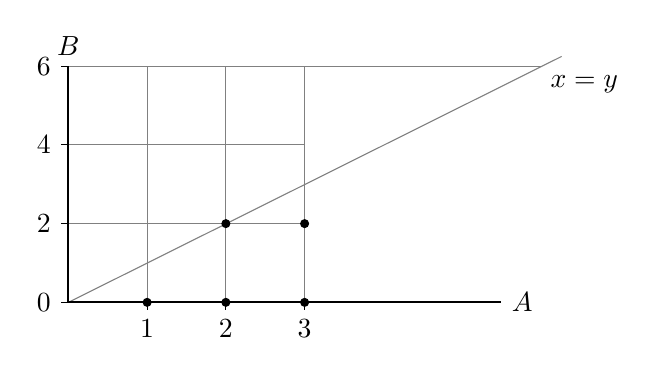
\begin{tikzpicture}
\foreach \x in {1,2,3}
\draw (\x,0.1) -- (\x,-0.1) node[below] {$\x$};

\foreach \x/\t in {0/0,1/2,2/4,3/6}
\draw (0.1,\x) -- (-0.1,\x) node[left] {$\t$};

\draw[color=gray] (0,1) -- (3,1);
\draw[color=gray] (0,2) -- (3,2);
\draw[color=gray] (1,0) -- (1,3);
\draw[color=gray] (2,0) -- (2,3);
\draw[color=gray] (3,0) -- (3,3);
\draw[color=gray] (0,0) -- (26.5:7);
\draw[color=gray] (0,3) -- (6,3) node[below right,color=black] {$x = y$};

\foreach \x/\y in {0/1,0/2,0/3,1/2,1/3}
\draw[fill=black] (\y,\x) circle (0.05);

\draw[thick] (0,3) node[above] {$B$} -- (0,0) -- (5.5,0) node[right] {$A$};
\end{tikzpicture}
